\chapter{Writing Custom User Modules}
\label{custommodules}
\index{modules, custom}

\section{Using the \texttt{DefaultGUIModel} Class}
\label{defaultGUImodules}
\index{DefaultGUIModel}
\index{modules, DefaultGUIModel}

User modules are implemented within RTXI as custom C\texttt{++} classes. The recommended way to create a module is to abstract from our provided base class named \texttt{DefaultGUIModel}. \texttt{DefaultGUIModel} constructs a simple graphical user interface (GUI) that allows users to interact with parameters and activate real-time code. Modules abstracted from it also inherit its methods for hard real-time execution and event handling, generating and accept signals, and capturing metadata automatically by the Data Recorder in HDF5 format. 

The following sections describe the \texttt{Neuron} module, a Hodgkin-Huxley model neuron class abstracted from DefaultGUIModel that generates a membrane voltage signal and accepts an optional external current input. The GUI consists of a column of textboxes and associated labels that display the module's parameters and internal state variables. Parameters are user-editable variables displayed in black, and internal state variables are intermediate computed values that cannot be edited manually by the user. States are shown in gray. Also, at the top left corner of the window is a unique instance ID that is given to each instantiated user module. This ID is important when connecting input and output from one module to another. 

\begin{figure}[h!] 
\begin{center}
\label{NeuronGUI}
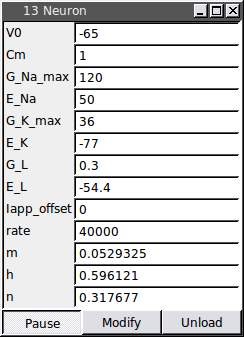
\includegraphics[width=2.1in]{hhneuron.png} 
\caption[The Neuron module's GUI]{The \texttt{Neuron} module is a Hodgkin-Huxley model neuron described by conductance-based differential equations. This GUI provides an interface by which a user can modify parameters, such as the conductance of the ion channels, on-the-fly and start and stop real-time execution of the module} 
\end{center}
\end{figure}

\subsection{Creating your own module class}

The quickest way to create a new user module is to duplicate an existing module directory and rename the files and the class. This involves renaming the class header (*.h) file, the class implementation (*.cpp) file, editing the Makefile and editing any instances of the old class name within each of these files. The latter include the class name, scope names, the constructor, and the deconstructor. A template user module is available online at \texttt{https://github.com/RTXI/plugin-template.git}.

Alternatively, you can browse through our module repository on GitHub (\texttt{https://github.com/RTXI/}) to find modules that perform functions similar to those desired. All our code is open-source, so you are free to fork our existing code and reconfigure it to meet your needs. 

\subsection{Edit the Makefile}
The Makefile instructs the compiler how to build your module and link it to RTXI. In RTXI v1.2 and later, the Makefile allows modules to be compiled outside the core RTXI source tree. The following sample Makefile installs a plugin called \texttt{my\_plugin} with dependencies \texttt{included\_class.h} and its source \texttt{included\_class.cpp}. 
\begin{maxipage}\index{Makefile}
\begin{example}
PLUGIN\_NAME = my\_plugin  \\
\vspace{.5cm}
HEADERS = my\_plugin.h  \\
\vspace{.5cm}
SOURCES = my\_plugin.cpp $\backslash$ \\
\hspace{2cm}included\_class.h $\backslash$ \\
\hspace{2cm}included\_class.cpp\\
\vspace{.5cm}
LIBS = -lgsl
\vspace{.5cm}
\#\#\# Do not edit below this line \#\#\# \\
include \$(shell rtxi\_plugin\_config --pkgdata-dir)/Makefile.plugin\_compile
\end{example}
\end{maxipage}

The \texttt{PLUGIN\_NAME} is the name of the shared object library (*.so) file when it is compiled. All modules should be given unique names because the compilation process will automatically overwrite identically-named modules. The \texttt{HEADERS} and \texttt{SOURCES} should also be edited to reflect the new source file names. For simple modules based on a single class, a single header and source file is all that is needed. You may base your module on additional custom classes whose sources must then be included here as well. The \texttt{LIBS} flag is used for any additional library flags. Here, \texttt{-lgsl} links this module against the GNU Scientific Library.

\subsection{Define model parameters, inputs, and outputs}

\texttt{DefaultGUIModel} uses a special workspace variable \texttt{vars[]} to define quantities in the module. The declaration of these types follows a simple syntax. Every \texttt{DefaultGUIModel} \attention module must have a workspace variable of type \texttt{variable\_t} as shown in the \texttt{vars[]} of the Neuron module. 

\begin{maxipage}
\begin{example}
static DefaultGUIModel::variable\_t vars$\left[\right]$ =\\
\{\\
\hspace{.5cm}\{"Iapp", "A", DefaultGUIModel::INPUT,\},\\
\hspace{.5cm}\{"Vm", "V", DefaultGUIModel::OUTPUT,\},\\
\hspace{.5cm}\{"V0", "mV", DefaultGUIModel::PARAMETER|DefaultGUIModel::DOUBLE,\},\\
\hspace{.5cm}\{"Cm", "uF/cm$^{\wedge}$2", DefaultGUIModel::PARAMETER|DefaultGUIModel::DOUBLE,\},\\
\hspace{.5cm}\{"G\_Na\_max", "mS/cm$^{\wedge}$2", DefaultGUIModel::PARAMETER|DefaultGUIModel::DOUBLE,\},\\
\hspace{.5cm}\{"E\_Na", "mV", DefaultGUIModel::PARAMETER|DefaultGUIModel::DOUBLE,\},\\
\hspace{.5cm}\{"G\_K\_max", "mS/cm$^{\wedge}$2", DefaultGUIModel::PARAMETER|DefaultGUIModel::DOUBLE,\},\\
\hspace{.5cm}\{"E\_K", "mV", DefaultGUIModel::PARAMETER|DefaultGUIModel::DOUBLE,\},\\
\hspace{.5cm}\{"G\_L", "mS/cm$^{\wedge}$2", DefaultGUIModel::PARAMETER|DefaultGUIModel::DOUBLE,\},\\
\hspace{.5cm}\{"E\_L", "mV", DefaultGUIModel::PARAMETER|DefaultGUIModel::DOUBLE,\},\\
\hspace{.5cm}\{"rate", "Hz",  DefaultGUIModel::PARAMETER|DefaultGUIModel::UINTEGER,\},\\
\hspace{.5cm}\{"m" "Sodium Activation", DefaultGUIModel::STATE,\},\\
\hspace{.5cm}\{"h", "Sodium Inactivation", DefaultGUIModel::STATE,\},\\
\hspace{.5cm}\{"n", "Potassium Activation", DefaultGUIModel::STATE,\},\\
\};
\end{example}
\end{maxipage}

Each element in \texttt{vars[]} defines an \texttt{INPUT}, \texttt{OUTPUT}, \texttt{PARAMETER}, \texttt{STATE} variable, or \texttt{COMMENT} for the module.  The first argument for each element is the label for the textbox in the GUI. This does not have to be the same as the variable name you use in the code to actually store the parameter value. The second argument is displayed as a Tooltip when you use your mouse to hover the cursor over that entry in the GUI. Enter any descriptive information here about the variable, such as an expanded form of your text label or the correct units of measurement. The third argument defines the variable as an input, output, etc. Notice that for parameters, you can also specify whether it is a double or integer numeric type. 

Declaring an \texttt{INPUT} creates a slot for your module to acquire data from the DAQ card or from another module. An \texttt{OUTPUT} creates a signal that is emitted from your module that can be sent to your DAQ card or any other module. These inputs and outputs can be directed from the Connector or the Data Recorder modules. In the Neuron module below, there is only one input, Iapp, and its value is accessed as the variable \texttt{input(0)}. If additional inputs had been declared, they would be accessed as \texttt{input(1)}, \texttt{input(2)}, and so on. The same rules apply for outputs. 

\texttt{STATE} variables and \texttt{PARAMETER}s are numeric datatypes. State variables are internal model variables that cannot be modified by the user through the GUI. Their values may be constant or they may change over time. Use a \texttt{STATE} to track the values of intermediate or computed quantities that can then be saved via the Data Recorder. A \texttt{PARAMETER} will accept user input through the GUI and can be modified on-the-fly during real-time execution. State variables and parameters appear in the GUI in the order that they are declared. In the example code, this mechanism is used to monitor the ion channel's activation variables, which are dependent on membrane voltage and integrated in real-time. A \texttt{COMMENT} is similar to a \texttt{PARAMETER}, but is used to store text strings such as information about the experiment that you would like to log. These are saved to the Data Recorder just like parameters, but should not be modified in real-time during model execution.

\attention If your parameter name contains a forward slash ``/", its values will not be automatically saved by the Data Recorder. This is a limitation of the HDF5 file format, which uses a directory-like syntax for specifying the data structure.

\subsection{Initialize the model}

The next section is the model constructor. If you changed the class name, this would read ``\texttt{YOURMODEL::YOURMODEL}". You can set the text that will appear in the title bar of your module window using the first argument of the constructor method. \attention The next required line is a call to the \texttt{createGUI()} function which generates the GUI shown in Figure \ref{NeuronGUI}. In this section, you should initialize all the variables and parameter values and make sure that the GUI reflects the actual values that are being used. In this example, much of this code is performed by the \seealso{Chapter \ref{DefaultGUIModel update}\\\texttt{update()}} \texttt{update()} function under the \texttt{INIT} flag. In other modules downloadable from our website, you will find a separate \texttt{initParameters()} function that handles all variable initializations. 

It is convenient to perform unit conversions when calling these functions so that the GUI accepts input in more user-friendly units. Finally, you should call \texttt{refresh()} to update the GUI to reflect your changes. The GUI textboxes will be initialized to the current values of the variables and \texttt{STATE} variables will be updated periodically during model execution. 
\begin{maxipage}
\begin{example}
Neuron::Neuron(void) : DefaultGUIModel("Neuron", ::vars, ::num\_vars) $\{$\\
\hspace{.5cm}createGUI(vars, num\_vars); // creates the GUI\\ 
\hspace{.5cm}V = V0;\\
\hspace{.5cm}m = m\_inf(V0);\\
\hspace{.5cm}h = h\_inf(V0);\\
\hspace{.5cm}n = n\_inf(V0);\\
\hspace{.5cm}period = RT::System::getInstance()->getPeriod() * 1e-6; // convert ns to ms\\
\hspace{.5cm}update(INIT); // calls the update() function with the INIT flag\\
\hspace{.5cm}refresh(); // refreshes the GUI to reflect parameter values stored in variables\\
$\}$
\end{example}
\end{maxipage}

Notice the method for retrieving the real-time period (sampling rate) of the system:
\begin{example}\index{RT::System::getInstance()-$>$getPeriod()}
RT::System::getInstance()->getPeriod();
\end{example}

This returns the period in nanoseconds. 


\subsection{The execute() loop}
\label{DefaultGUIModel execute}
The \texttt{execute()} function will run to completion on every time step. The computations performed here must complete within the real-time period that you have set in the \seealso{Chapter \ref{system control panel} \\System Control Panel}System Control panel to maintain system stability. The efficiency of your code here will affect the performance of your system. You should use private variables defined in the class header rather than creating variables inside the function on every time step. If you absolutely must create a variable inside \texttt{execute()}, use a static call so that the same memory block is used each time. \attention You should be wary of using \texttt{do-while} and \texttt{for} structures if you are uncertain how long these loops will take to complete. Within the execute function, you must also be careful to bound the output signal and perform your own error checking to maintain the stability of the closed-loop. Notice that at the end, we have set \texttt{output(0)} to update the membrane voltage signal emitted by this module. RTXI's signals-and-slots architecture allows you to \attention connect any signal to any slot. There is no error checking that the connection is valid, eg. that quantities with matching units of measurement are connected.

\bigskip\hrule
\begin{example}
void Neuron::execute(void) $\{$\\
\hspace{.5cm}for (int i = 0; i < steps; ++i)\\
\hspace{1cm}solve(period / steps, y); // integrate equations\\
\hspace{.5cm}output(0) = V * 1e-3; // convert to mV\\
$\}$\\
\end{example}
\bigskip
\hrule

\subsection{The update() function}
\label{DefaultGUIModel update}

The \texttt{update{}} function implemented in \texttt{DefaultGUIModel} that is designed to handle function calls depending on the state of the GUI. It provides several flags to help organize code and handle events in modules. 
\begin{itemize}
\item \texttt{INIT}: non-event related but useful for placing code to initialize the model
\item \texttt{MODIFY}: called when the "Modify" button is pressed in the GUI
\item \texttt{PAUSE}: called when the model is paused
\item \texttt{UNPAUSE}: called when the model is unpaused
\label{pause flag}\item \texttt{PERIOD}: called when the real-time period of the system is changed
\end{itemize}

Under the \texttt{INIT} flag, you should initialize any variables or GUI settings that were not already addressed in the constructor. To assign a variable as a \texttt{STATE} variable in the GUI, use:

\begin{example}\index{setState()}
setState("YOUR\_GUI\_LABEL", YOUR\_VARIABLE);
\end{example}

\attention \texttt{YOUR\_GUI\_LABEL} must exactly match the label that you set in \texttt{variable\_t vars$\left[\right]$} above. 

Similarly, you initialize the GUI for a \texttt{PARAMETER} with:
\begin{example}\index{setParameter()}
setParameter("YOUR\_GUI\_LABEL", YOUR\_VARIABLE);
\end{example}

It is often the case that you may want to display units in the GUI with more convenient physiological units of measurement, eg. mV instead of V. In that case, you can call the function as follows:
\begin{example}\index{setParameter()}
setParameter("E\_Na", E\_Na*1000); // convert to mV\\
\end{example}

\attention Always comment your units. Otherwise, your code will not be readily readable by other or even yourself later on, 

Under the \texttt{MODIFY} flag, you should grab all the values in the GUI textboxes and update the values of the parameters as follows:
\begin{example}
YOUR\_VARIABLE = getParameter("YOUR\_GUI\_LABEL").toDouble();
\end{example}

If you do any unit conversions with \texttt{setParameter()}, make sure you do the inverse with \texttt{getParameter()}. You may also want to add code to the \texttt{PAUSE} flag to set the output of your module to zero, e.g. the amplitude of an injected current. \attention In some cases, you will want to reset certain internal variables when you stop or start the model eg. a counter that keeps track of your model execution time. Under the \texttt{PERIOD} flag, you will always want to update your model with the new real-time period. 

\begin{maxipage}
\begin{example}
void Neuron::update(DefaultGUIModel::update\_flags\_t flag) $\{$\\
\hspace{.5cm}switch (flag) $\{$\\
\hspace{1cm}case INIT:\\
\hspace{1.5cm}setState("m", m);\\
\hspace{1.5cm}setState("h", h);\\
\hspace{1.5cm}setState("n", n);\\
\hspace{1.5cm}setParameter("V0", V0);\\
\hspace{1.5cm}setParameter("Cm", Cm);\\
\hspace{1.5cm}setParameter("G\_Na\_max", G\_Na\_max);\\
\hspace{1.5cm}setParameter("E\_Na", E\_Na);\\
\hspace{1.5cm}setParameter("G\_K\_max", G\_K\_max);\\
\hspace{1.5cm}setParameter("E\_K", E\_K);\\
\hspace{1.5cm}setParameter("G\_L", G\_L);\\
\hspace{1.5cm}setParameter("E\_L", E\_L);\\
\hspace{1.5cm}setParameter("Iapp\_offset", Iapp\_offset);\\
\hspace{1.5cm}setParameter("rate", rate);\\
\hspace{1.5cm}break;\\
\hspace{1cm}case MODIFY:\\
\hspace{1.5cm}V0 = getParameter("V0").toDouble();\\
\hspace{1.5cm}Cm = getParameter("Cm").toDouble();\\
\hspace{1.5cm}G\_Na\_max = getParameter("G\_Na\_max").toDouble();\\
\hspace{1.5cm}E\_Na = getParameter("E\_Na").toDouble();\\
\hspace{1.5cm}G\_K\_max = getParameter("G\_K\_max").toDouble();\\
\hspace{1.5cm}E\_K = getParameter("E\_K").toDouble();\\
\hspace{1.5cm}G\_L = getParameter("G\_L").toDouble();\\
\hspace{1.5cm}E\_L = getParameter("E\_L").toDouble();\\
\hspace{1.5cm}Iapp\_offset = getParameter("Iapp\_offset").toDouble();\\
\hspace{1.5cm}rate = getParameter("rate").toDouble();\\
\hspace{1.5cm}steps = static\_cast (ceil(period * rate / 1000.0));\\
\hspace{1.5cm}V = V0;\\
\hspace{1.5cm}m = m\_inf(V0);\\
\hspace{1.5cm}h = h\_inf(V0);\\
\hspace{1.5cm}n = n\_inf(V0);\\
\hspace{1.5cm}break;\\
\hspace{1cm}case PAUSE:\\
\hspace{1.5cm}break;\\
\hspace{1cm}case UNPAUSE:\\
\hspace{1.5cm}break;\\
\hspace{1cm}case PERIOD:\\
\hspace{1.5cm}period = RT::System::getInstance()->getPeriod() * 1e-6; // ms\\
\hspace{1.5cm}steps = static\_cast (ceil(period * rate / 1000.0));\\
\hspace{1.5cm}break;\\
\hspace{1cm}default:\\
\hspace{1.5cm}break;\\
\hspace{.5cm}$\}$\\
$\}$
\end{example}
\end{maxipage}